\documentclass[a4paper, 12pt]{article}
\usepackage[a4paper,top=1.5cm, bottom=1.5cm, left=1cm, right=1cm]{geometry}
\usepackage{cmap}					% поиск в PDF
\usepackage{mathtext} 				% русские буквы в формулах
\usepackage[T2A]{fontenc}			% кодировка
\usepackage[utf8]{inputenc}			% кодировка исходного текста
\usepackage[english,russian]{babel}	% локализация и переносы

\usepackage{amsmath}
\usepackage{indentfirst}
\usepackage{longtable}
\usepackage{graphicx}
\usepackage{array}

\usepackage{wrapfig}
\usepackage{siunitx} % Required for alignment
\usepackage{subfigure}
\usepackage{multirow}
\usepackage{rotating}
\usepackage{caption}
\usepackage{subcaption}

\graphicspath{{img/}}


\title{\begin{center}Лабораторная работа №2.3.1\end{center}
Получение и измерение вакуума}
\author{Рожков А. В. \\ Преподаватель Яворский В. А.}
\date{\today}

\begin{document}
    \pagenumbering{gobble}
    \maketitle
    \newpage
    \pagenumbering{arabic}

    \textbf{Цель работы:} 1) измерение объёмов форвакуумной и высоковакуумной частей установки; 2) определение скорости откачки системы в стационарном режиме, а также по ухудшению и по улучшению вакуума.

    \textbf{В работе используются:} вакуумная установка с манометрами: масляным ($\sigma_h = 1 мм$), термопарным ПМТ-2 ($\varepsilon_{p} = 30\%$) и ионизационным ПМИ-2 ($\varepsilon_{p} = 35\%$).

    \section{Экспериментальная установка}

    \begin{figure}[h]
        \center{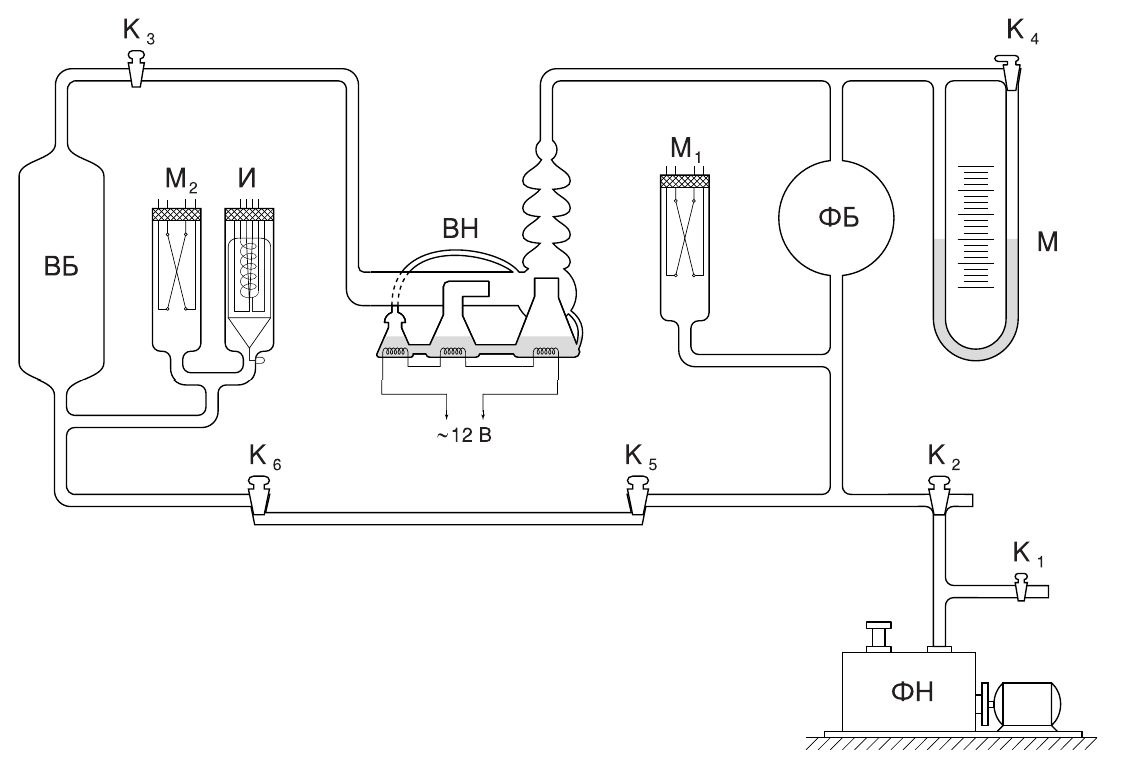
\includegraphics[width=0.8\textwidth]{ustanovka}}
        \caption{Схема экспериментальной установки.}
        \label{ris:ustanovka}
    \end{figure}

    \paragraph{}
    Установка изготовлена из стекла и состоит из форвакуумного баллона (ФБ), высоковакуумного диффузионного насоса (ВН), высоковакуумного баллона (ВБ), масляного (М) и ионизационного (И) манометров, термопарных манометров ($М_1$ и $М_2$), форвакуумного насоса (ФН) и соединительных кранов (Рис. \ref{ris:ustanovka}). Кроме того, в состав установки входят: вариатор (автотрансформатор с регулируемым выходным напряжением), или реостат и амперметр для регулирования тока нагревателя диффузионного насоса.

    \paragraph{Маслянный манометр:}
    Представляет собой U-образную трубку, до половины наполненную вязким маслом, обладающим весьма низким давлением насыщенных паров. Так как плотность масла мала, $\rho = 0,885 г/см^3$ , то при помощи манометра можно измерить только небольшие разности давлений (до нескольких торр). Во время откачки и заполнения установки атмосферным воздухом кран $К_4$ соединяющий оба колена манометра, должен быть открыт во избежание выброса масла и загрязнения установки. Кран $К_4$ закрывается только при измерении давления U-образным манометром.


    \newpage

    \paragraph{Термопарный манометр:}
    Чувствительным элементом манометра является термопара, заключенная в стеклянный баллон. Устройство термопары пояснено на (Рис. \ref{ris:termoparni_monometr}). По нити накала НН пропускается ток постоянной величины. Термопара ТТ присоединяется к милливольтметру, показания которого определяются температурой нити накала и зависят от отдачи тепла в окружающее пространство. Потери тепла определяются теплопроводностью нити и термопары, теплопроводностью газа, переносом тепла конвективными потоками газа внутри лампы и теплоизлучением нити (инфракрасное тепловое излучение). В обычном режиме лампы основную роль играет теплопроводность газа. При давлениях >1 торр теплопроводность газа, а вместе с ней и ЭДС термопары практически не зависят от давления газа, и прибор не работает. При улучшении вакуума средний свободный пробег молекул становится сравнимым с диаметром нити, теплоотвод падает и температура спая возрастает. При вакууме $~10^{-3}$ торр теплоотвод, осуществляемый газом, становится сравнимым с другими видами потерь тепла и температура нити становится практически постоянной. Градуировочная кривая термопарного манометра приведена на (Рис. \ref{ris:termopara_graduirovka}).

    \begin{figure}[h]
    \centering
    \begin{minipage}{0.3\textwidth}
        \centering
        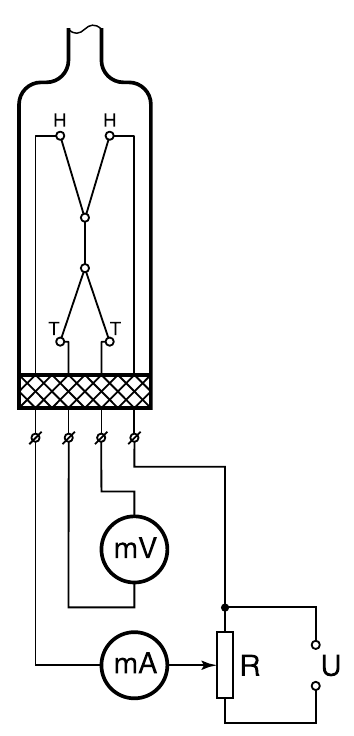
\includegraphics[width=0.9\textwidth]{termoparni_monometr}
        \caption{Схема термопарного манометра.}
        \label{ris:termoparni_monometr}
    \end{minipage}\hfill
    \begin{minipage}{0.7\textwidth}
        \centering
        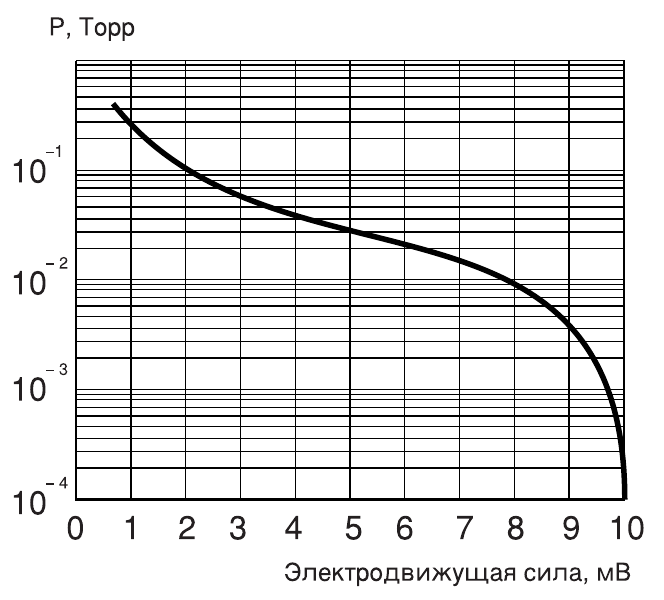
\includegraphics[width=0.9\textwidth]{termopara_graduirovka}
        \caption{Градуировочная кривая термопарного манометра.}
        \label{ris:termopara_graduirovka}
    \end{minipage}
    \end{figure}

    \newpage

    \paragraph{Ионизационный манометр:}
    Схема ионизационного манометра изображена на (Рис. \ref{ris:ionizacionni_monometr}). Он представляет собой трехэлектродную лампу. Электроны испускаются накаленным катодом и увлекаются электрическим полем к аноду, имеющему вид спирали. Проскакивая за ее витки,электроны замедляются полем коллектора и возвращаются к катоду, а от него вновь увлекаются к аноду. Прежде чем осесть на аноде, они успевают много раз пересечь пространство между катодом и коллектором. На своем пути электроны ионизуют молекулы газа. Ионы, образовавшиеся между анодом и коллектором, притягиваются полем коллектора и определяют его ток. Ионный ток в цепи коллектора пропорционален плотности газа и поэтому может служить мерой давления. Вероятность ионизации зависит от рода газа, заполняющего лампу (а значит, и откачиваемый объем). Калибровка манометра верна, если остаточным газом является воздух. Накаленный катод ионизационного манометра перегорает, если давление в системе превышает $10^{-3}$ торр. Поэтому включать ионизационный манометр можно, только убедившись по термопарному манометру, что давление в системе не превышает $10^{-3}$ торр. При измерении нить ионизационного манометра сильно греется. При этом она сама, окружающие ее электроды и стенки стеклянного баллона могут десорбировать поглощенные ранее газы. Выделяющиеся газы изменяют давление в лампе и приводят к неверным показаниям. Поэтому перед измерениями ионизационный манометр прогревается (обезгаживается) в течение 10–15 мин. Для прогрева пропускается ток через спиральный анод лампы.

    \vspace{1cm}

    \begin{figure}[h]
        \center{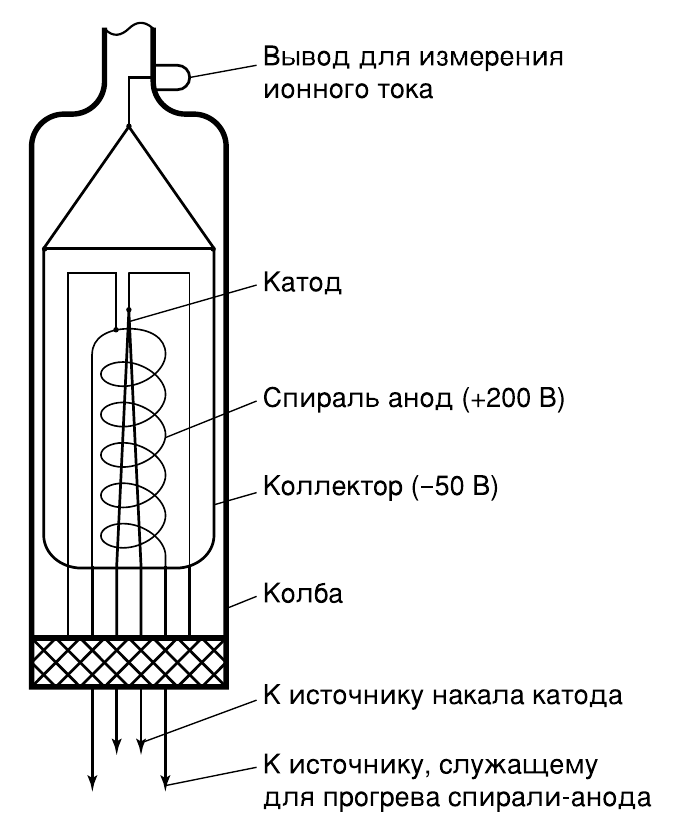
\includegraphics[width=0.5\textwidth]{ionizacionni_monometr}}
        \caption{Схема ионизационного манометра.}
        \label{ris:ionizacionni_monometr}
    \end{figure}

    \newpage

    \paragraph{Диффузионный насос:}
    Откачивающее действие диффузионного насоса основано на диффузии (внедрении) молекул разреженного воздуха в струю паров масла. Попавшие в струю молекулы газа увлекаются ею и уже не возвращаются назад. Устройство одной ступени масляного диффузионного насоса схематически показано на (Рис. \ref{ris:diffuzionni_nasos}) (в лабораторной установке используется несколько откачивающих ступеней). Масло, налитое в сосуд А, подогревается электрической печкой. Пары масла поднимаются по трубе Б и вырываются из сопла В. Струя паров увлекает молекулы газа,которые поступают из откачиваемого сосуда через трубку ВВ. Дальше смесь попадает в вертикальную трубу Г. Здесь масло осаждается на стенках трубы и маслосборников и стекает вниз, а оставшийся газ через трубу ФВ откачивается форвакуумным насосом. Диффузионный насос работает наиболее эффективно при давлении, когда длина свободного пробега молекул воздуха примерно равна ширине кольцевого зазора между соплом В и стенками трубы ВВ. В этом случае пары масла увлекают молекулы воздуха из всего сечения зазора. Давление насыщенных паров масла при рабочей температуре, создаваемой обогревателем сосуда А, много больше $5\cdot10^{-2}$ торр. Именно поэтому пары масла создают плотную струю, которая и увлекает с собой молекулы газа. Если диффузионный насос включить при давлении, сравнимом с давлением насыщенного пара масла, то последнее никакой струи не создаст и масло будет просто окисляться и угорать.

    Диффузионный насос, используемый в нашей установке, имеет две ступени и соответственно два сопла (Рис. \ref{ris:nasos_irl}). Одно сопло вертикальное (первая ступень), второе сопло горизонтальное (вторая ступень). За второй ступенью имеется еще одна печь, но пар из этой печи поступает не в сопло, а по тонкой трубке подводится ближе к печке первой ступени. Эта печь осуществляет фракционирование масла. Легколетучие фракции масла, испаряясь, поступают в первую ступень, обогащая ее легколетучей фракцией масла. По этой причине плотность струи первой ступени выше и эта ступень начинает откачивать при более высоком давлении в форвакуумной части установки. Вторая ступень обогащается малолетучими фракциями. Плотность струи второй ступени меньше, но меньше и давление насыщенных паров масла в этой ступени. Соответственно в откачиваемый объем поступает меньше паров масла и его удается откачать до более высокого вакуума, чем если бы мы работали только с одной ступенью.


    \begin{figure}[h]
    \centering
    \begin{minipage}{0.35\textwidth}
        \centering
        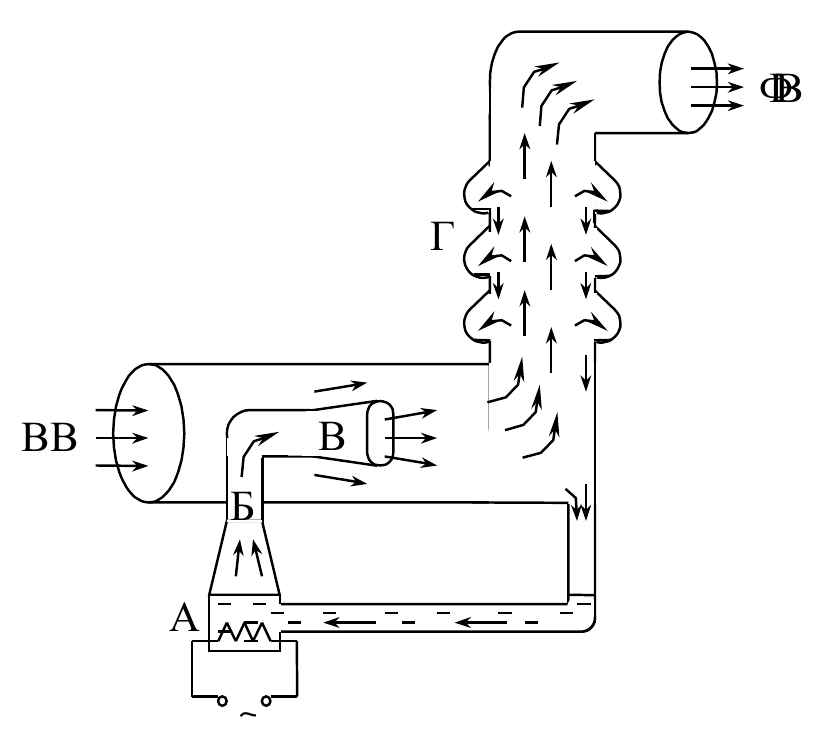
\includegraphics[width=1\textwidth]{diffuzionni_nasos}
        \caption{Схема одной ступени диффузионного насоса.}
        \label{ris:diffuzionni_nasos}
    \end{minipage}\hfill
    \begin{minipage}{0.65\textwidth}
        \centering
        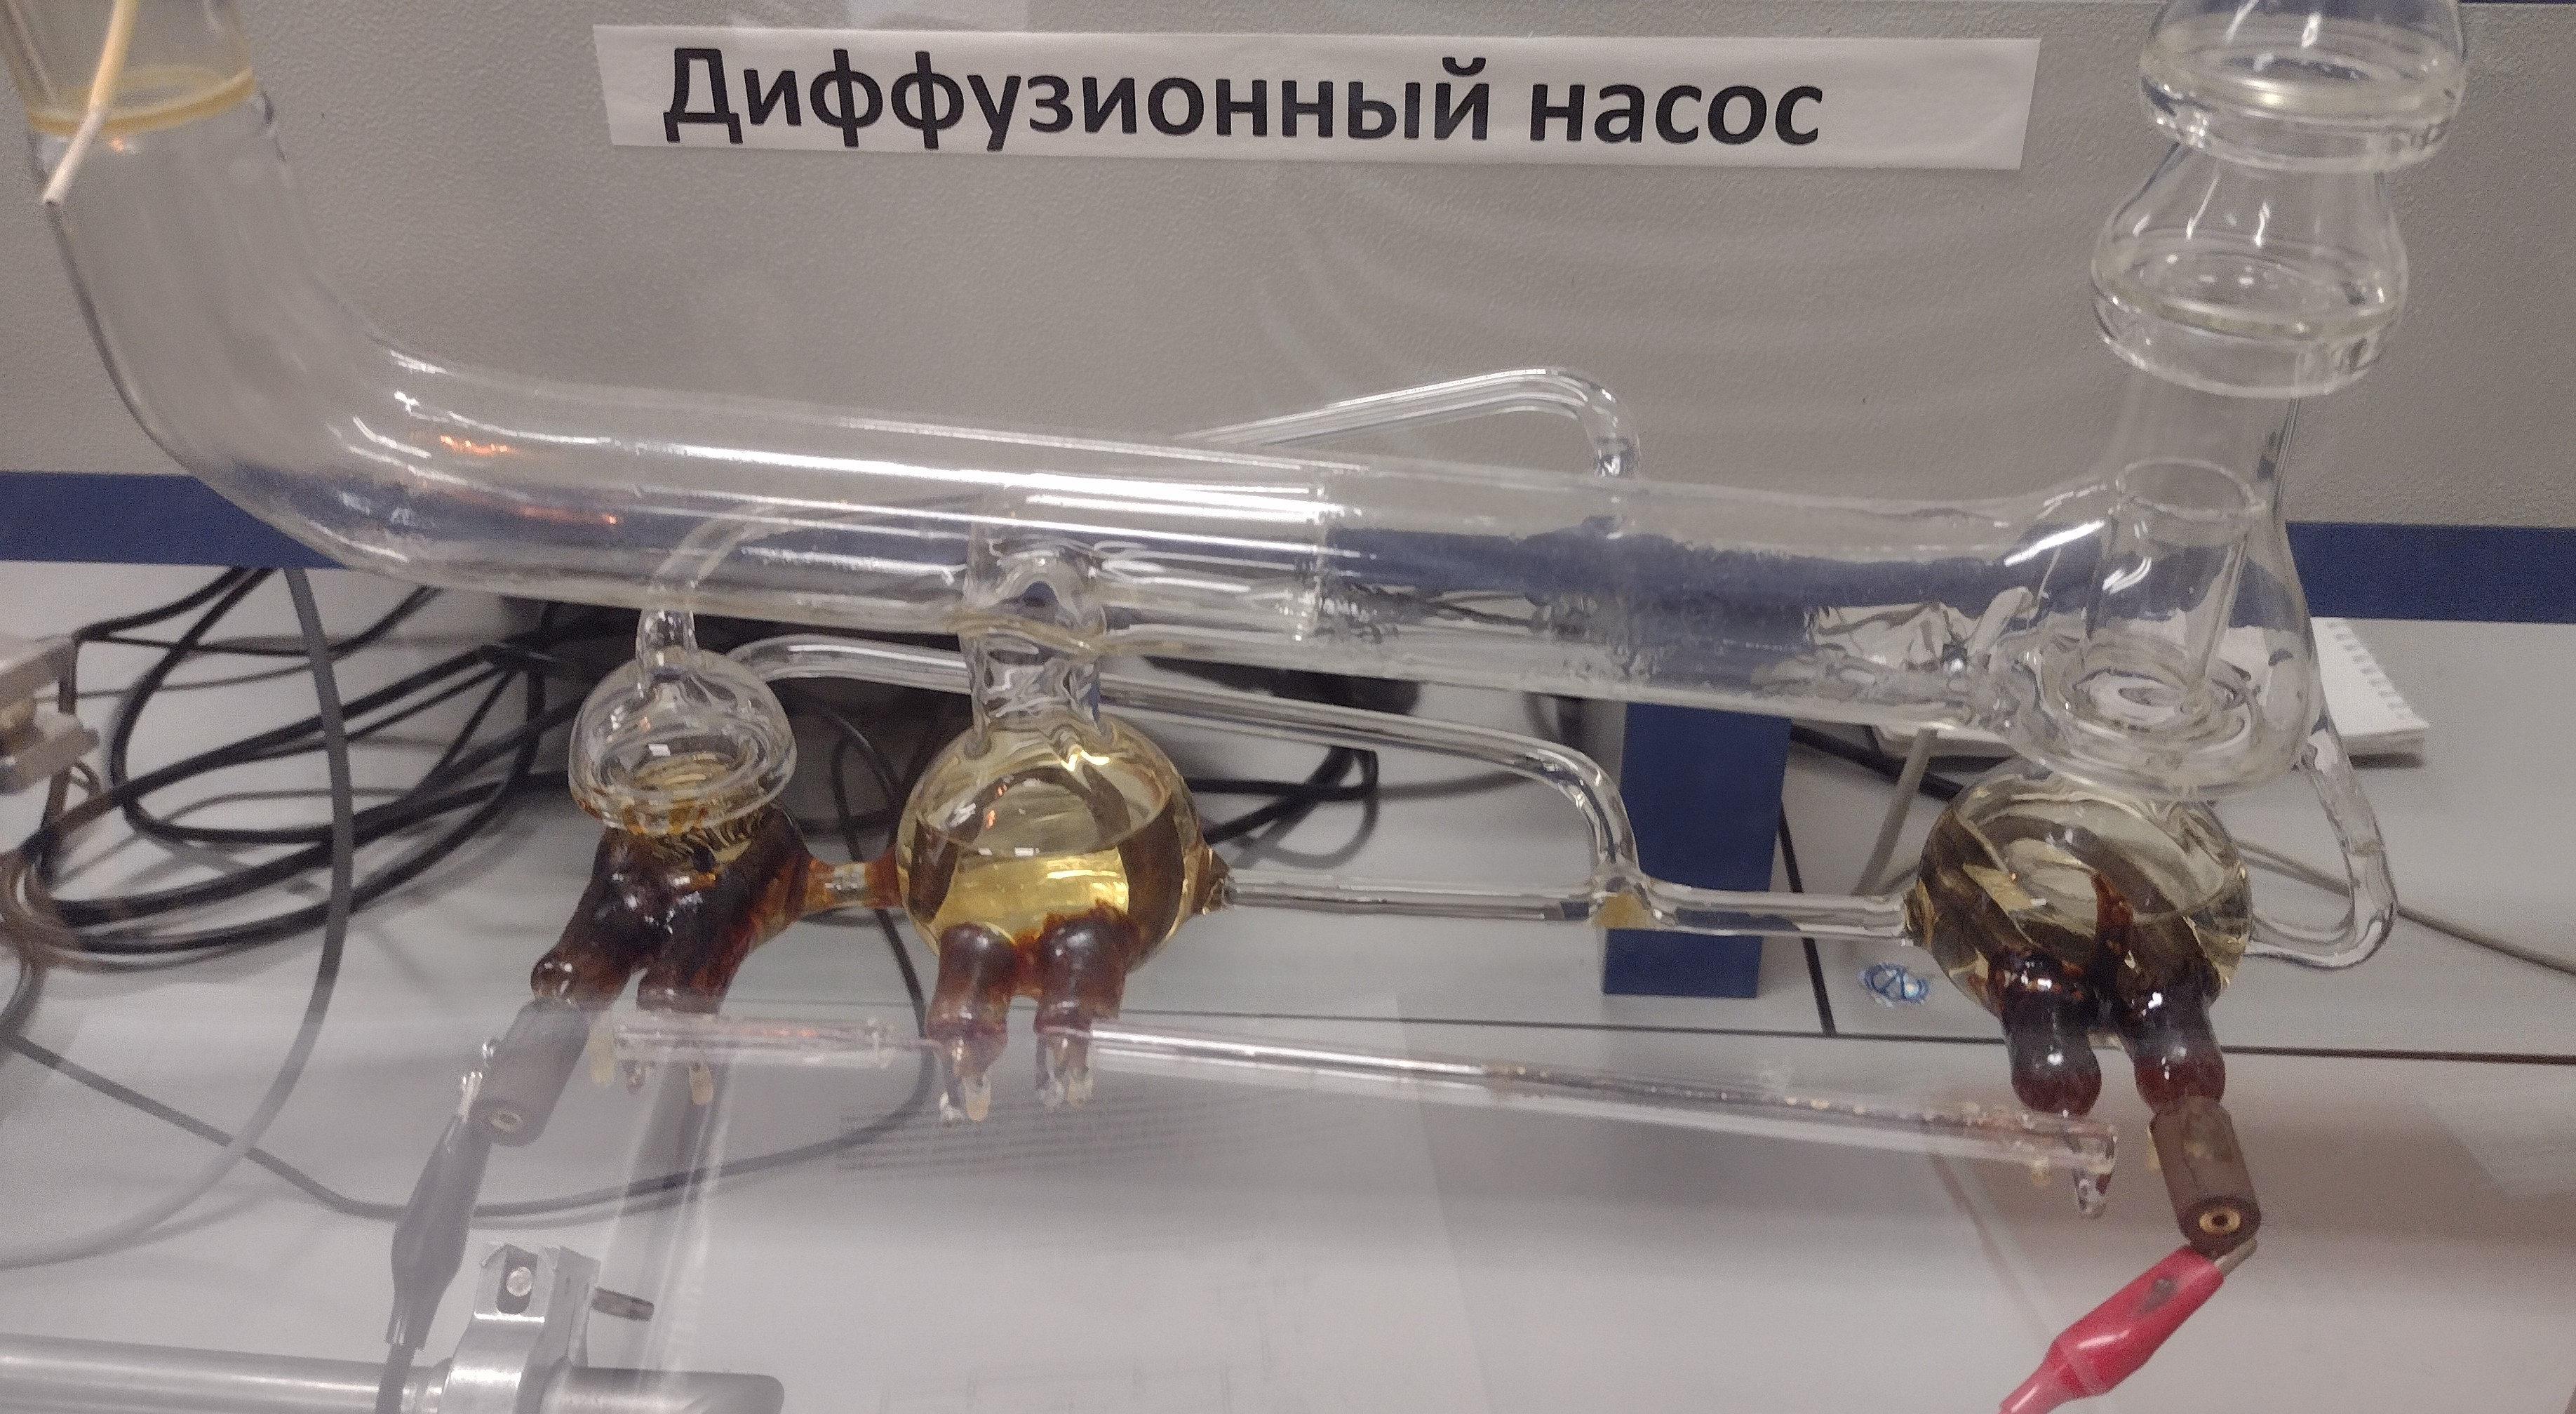
\includegraphics[width=0.9\textwidth]{nasos_irl}
        \caption{Диффузионный насос используемый в нашей работе.}
        \label{ris:nasos_irl}
    \end{minipage}
    \end{figure}


    \section{Теоретическая часть}

    \paragraph{Процесс откачки: }
    Производительность насоса определяется скоростью откачки $W$ (л/с): W — это объем газа, удаляемого из сосуда при данном давлении за единицу времени. Скорость откачки форвакуумного насоса равна емкости воздухозаборной камеры, умноженной на число оборотов в секунду.

    Обозначим через $Q_д$ количество газа, десорбирующегося с поверхности откачиваемого объема в единицу времени, через $Q_и$ -- количество газа, проникающего в единицу времени в этот объем извне -- через течи. Будем считать, что насос обладает скоростью откачки $W$ и в то же время сам является источником газа; пусть $Q_н$ — поток газа, поступающего из насоса назад в откачиваемую систему. $Q=Q_д + Q_и + Q_н$ измеряем в единицах (моль/с). Получаем формулу
    \begin{equation*}
        -\frac{VdP}{RT}=\left(\frac{PW}{RT} - Q\right)dt
    \end{equation*}
    При предельном давлении $dP=0$ и поэтому получаем
    \begin{equation*}
        Q=\frac{P_{пр}W}{RT}
    \end{equation*}
    Подставляя получаем
    \begin{equation*}
        -VdP=W(P-P_{пр})dt
    \end{equation*}
    Интегрируем полученное ур-е и получаем
    \begin{equation}
        P-P_{пр}=(P_0 - P_{пр})\exp\left(-\frac{W}{V}t\right)
    \end{equation}
    Пренебрегая $P_{пр}$ относительно $P_0$
    \begin{equation}
        P=P_0\exp\left(-\frac{W}{V}t\right) \label{W}
    \end{equation}
    Как видим, величина $\tau=V/W$ показывает характерное время откачки системы.

    Теперь попробуем понять чем обусловлена скорость откачки. Очевидно, скорость $W$ зависит от скорости откачки насоса $W_н$, но она так же зависит от трубопровода соединяющего насос к откачиваемой части, т.к. если трубопровод не сможет обеспечить достаточное количество газа к входу насоса то, производительность упадет.

    \begin{figure}[h]
        \center{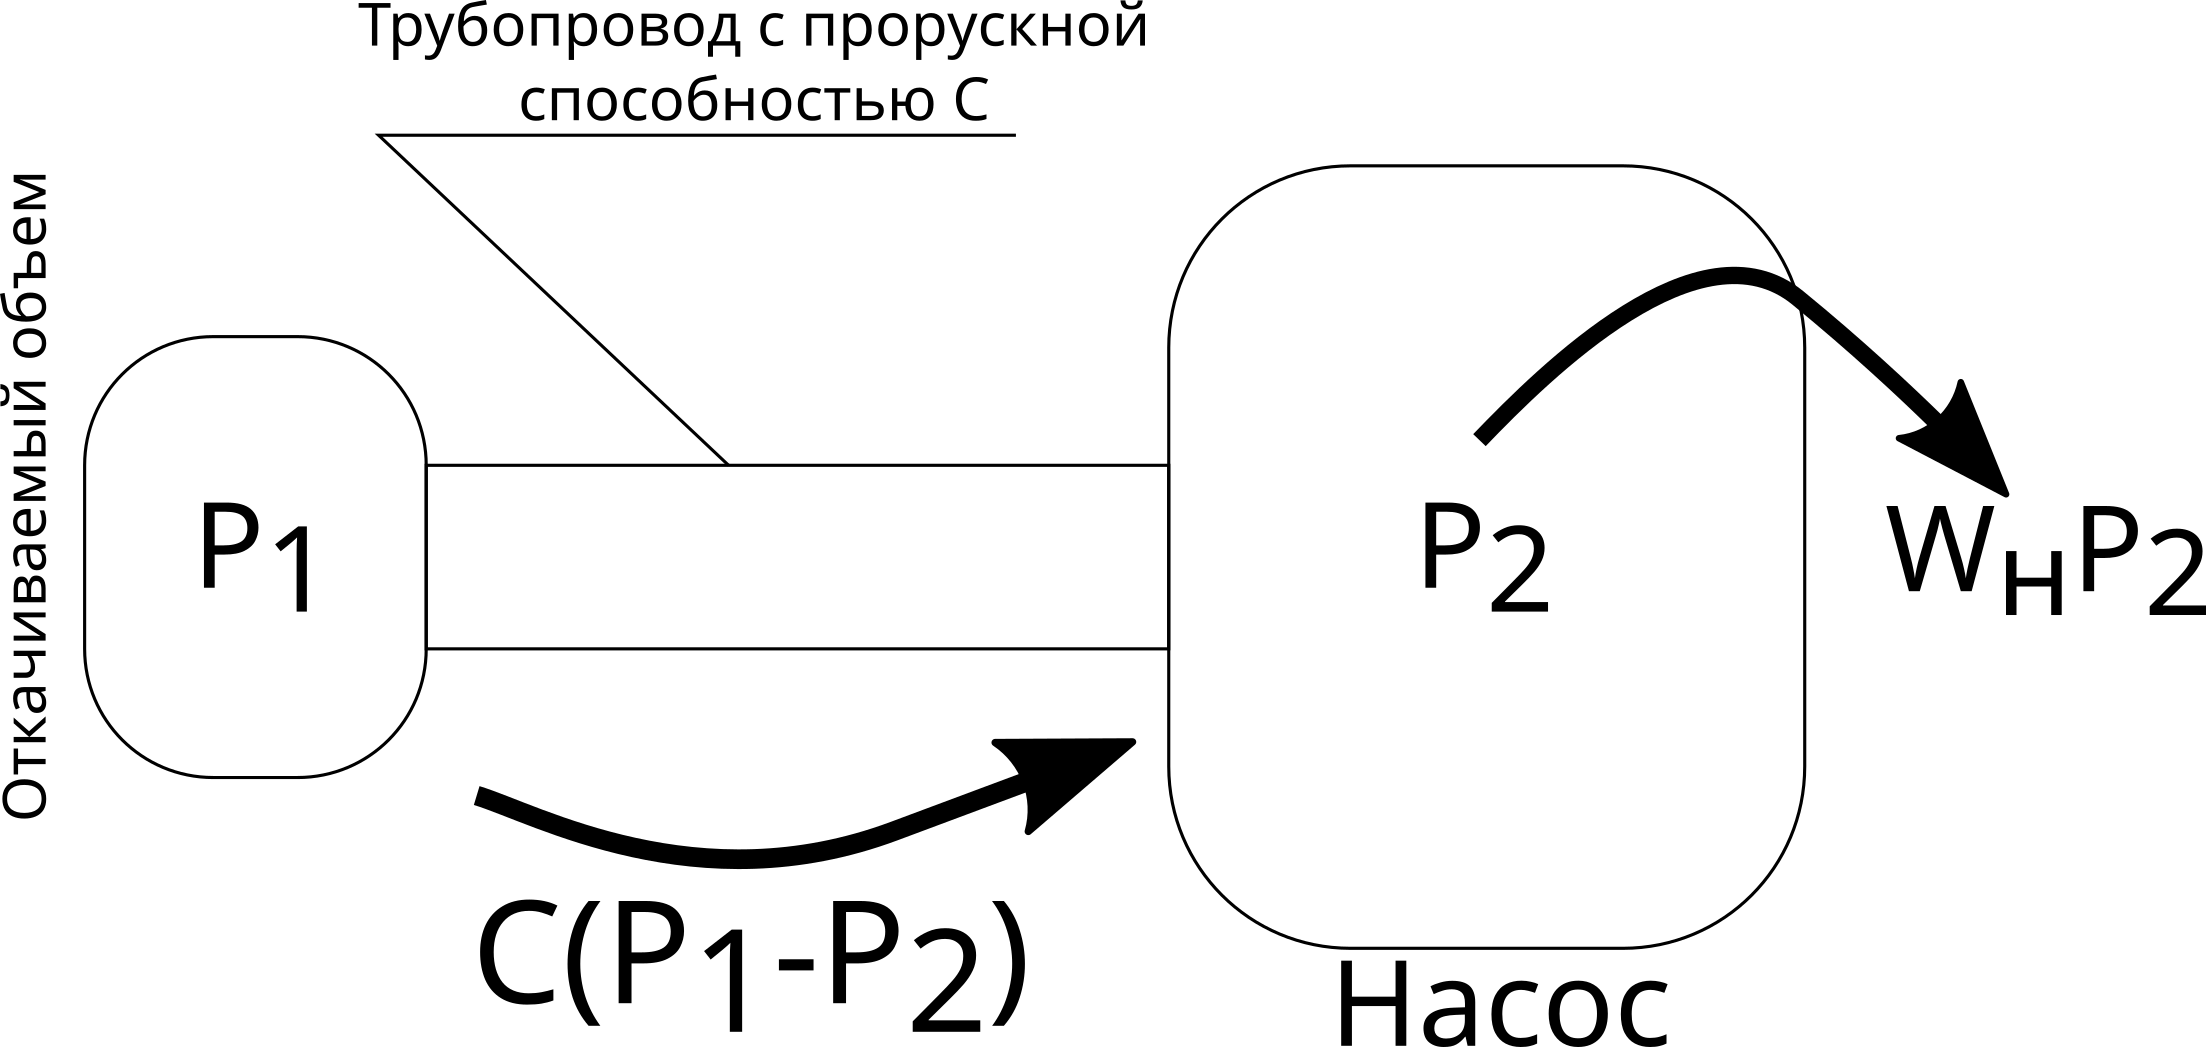
\includegraphics[width=0.7\textwidth]{nasos_sketch}}
        \caption{Схема насоса с трубопроводом.}
        \label{ris:nasos_sketch}
    \end{figure}
    Попробуем описать систему математически. Пусть у нас есть насос со скоростью откачки $W_н$ и трубопровод с пропускной способностью $C$. Давление в откачиваемом объеме -- $P_1$. Исследовав схему \ref{ris:nasos_sketch} получаем

    \begin{equation*}
        C(P_1 - P_2)=W_нP_2 \Rightarrow P_2=\frac{CP_1}{C+W_н} \Rightarrow WP_1=W_нP_2=\frac{CW_н}{C+W_н}P_1
    \end{equation*}
    Как видим, для результирующей скорости $W$ верно соотношение

    \begin{equation*}
        \frac{1}{W} = \frac{1}{W_н} + \frac{1}{C}
    \end{equation*}
    Обобщая это выражение для последовательно соединенных труб получаем

    \begin{equation}
        \frac{1}{W} = \frac{1}{W_н} + \frac{1}{C_1} + \frac{1}{C_2} + ...
        \label{resulting_speed}
    \end{equation}
    Заметим только что данные формулировки верны при молекулярном режиме течения, когда вязкое трение не имеет большого вклада в движение газа.

    \paragraph{Течение газа через трубу:} Для количества газа, протекающего через трубу в условиях высокого вакуума или, как говорят, в кнудсеновском режиме, справедлива формула

    \begin{equation}
        \frac{d(PV)}{dt} = \frac{4}{3}r^3 \sqrt{\frac{2\pi RT}{\mu}} \frac{P_2 - P_1}{L}
        \label{prop_spos_truba}
    \end{equation}
    где $r$ и $L$ соответственно радиус и длина трубы. Если пренебречь давлением $P_1$ у конца, обращенного к насосу, получаем формулу для пропускной способности трубы
    \begin{equation}
    C_{тр} = \frac{dV}{dt} = \frac{4}{3}\frac{r^3}{L}\sqrt{\frac{2\pi RT}{\mu}} \label{C_trubki}
    \end{equation}
    Для пропускной способности отверстия (например в кранах) имеем формулу

    \begin{equation}
    C_{отв}=S\frac{\bar v}{4}
    \end{equation}

    \section{Ход работы}
    \subsection{Определение объёма форвакуумной и высоковакуумной частей установки}
        \subsubsection{Открываем все краны установки}

        \subsubsection{Впускаем в установку атмосферный воздух}

        \subsubsection{Изолируем объём капилляра.}

            $V_{кап} = (50 \pm 1) см^3$

        \subsubsection{Закрываем кран, соединяющий установку с атмосферой, и кран между установкой и форвакуумным насосом. Включаем форвакуумный насос}

            В течение 2 минут насос откачивает сам себя и патрубок установки.

        \subsubsection{Открываем кран и откачиваем установку}

        \subsubsection{Включаем вакуумметры в сеть}

            При достижении давления $ 1.9*10^{-2}~мм.рт.ст $ останавливаем процесс откачки.

        \subsubsection{Отсоединяем установку от форвакуумного насоса}

        \subsubsection{Отсоединяем высоковакуумную часть установки от форвакуумной}

        \subsubsection{Закрыв кран, вводим в работу масляный манометр}

        \subsubsection{Выпускаем запертый в капилляре воздух в установку}

        \subsubsection{Выпущенный воздух повышает давление в установке}

            Это давление измеряется масляным манометром.

            Верхнее значение: $h_1 = (34.6 \pm 0.1)~см.масл.ст$

            Нижнее значение:  $h_2 = (5.4 \pm 0.1)~см.масл.ст$

            Разность уровней: $\Delta h_{фв} = (29.2 \pm 0.2)~см.масл.ст$

        \subsubsection{Находим объём форвакуумной части установки}

            Пренебрегаем остаточным давлением $1.9*10^{-2}~мм.рт.ст$, так как оно в $\sim1000$ раз меньше остальных давлений.

            \begin{align*}
                P_{атм} &= (100.43 \pm 0.01)~кПа & \rho_{масла} &= (0.885 \pm 0.001)~г/см^3
            \end{align*}

            \begin{align*}
                V_{фв} &= \frac{P_{атм} V_{кап}}{P_{манометра}} = \frac{P_{атм} V_{кап}}{\rho_{масла} g \Delta h_{фв}} = 1980~см^3\\\\
                \sigma_{V_{фв}} &= V_{фв} \sqrt{\left( \frac{\sigma_{P_{атм}}}{P_{атм}} \right)^2 + \left( \frac{\sigma_{V_{кап}}}{V_{кап}} \right)^2 + \left( \frac{\sigma_{\rho_{масла}}}{\rho_{масла}} \right)^2 + \left( \frac{\sigma_{g}}{g} \right)^2 + \left( \frac{\sigma_{\Delta h_{фв}}}{\Delta h_{фв}} \right)^2} = 50~см^3
            \end{align*}

        \subsubsection{Находим объём всей установки}

            Для этого открываем кран, соединяющий высоковакуумную и форвакуумную части и по показаниям масляного манометра аналогично вычисляем полный объём обоих частей.

            Верхнее значение: $h_2 = (11.0 \pm 0.1)~см.масл.ст$

            Нижнее значение:  $h_3 = (29.7 \pm 0.1)~см.масл.ст$

            Разность уровней: $\Delta h_{полн} = (18.7 \pm 0.2)~см.масл.ст$

            \begin{align*}
                V_{полн} &= \frac{P_{атм} V_{кап}}{P_{манометра}} = \frac{P_{атм} V_{кап}}{\rho_{масла} g \Delta h_{полн}} = (3096 \pm 80)~см^3\\\\
            \end{align*}

        \subsubsection{Открываем кран масляного манометра, чтобы избежать переброса масла в установку}

        \subsubsection{Находим объём высоковакуумной части установки}

            \begin{align}
                V_{вв} &= V_{полн} - V_{фв} = 1113~см^3\\
                \sigma_{V_{вв}} &= \sqrt{ \sigma_{V_{полн}}^2 + \sigma_{V_{фв}}^2 } = 90~см^3
            \end{align}

    \subsubsection{Повторяем измерения ещё раз}

        Результаты приведены в таблице \ref{volumes}

        \begin{table}[!ht]
            \centering
            \begin{tabular}{|l|c|c|}
                \hline

                 & Изм. 1 & Изм. 2\\ \hline
                $h_1, см$ & $(34.6 \pm 0.1)$ & $(34.7 \pm 0.1)$\\ \hline
                $h_2, см$ & $(5.4 \pm 0.1)$ & $(5.2 \pm 0.1)$\\ \hline
                $\Delta h_{фв}$ & $(29.2 \pm 0.2)$ & $(29.5 \pm 0.2)$\\ \hline
                $h_3, см$ & $(29.7 \pm 0.1)$ & $(29.5 \pm 0.1)$\\ \hline
                $h_4, см$ & $(11.0 \pm 0.1)$ & $(10.9 \pm 0.1)$\\ \hline
                $\Delta h_{полн}$ & $(18.7 \pm 0.2)$ & $(18.6 \pm 0.2)$\\ \hline
                $V_{фв}$ & $(1980.0 \pm 50.0)$ & $(1960.0 \pm 50.0)$\\ \hline
                $V_{вв}$ & $(1110.0 \pm 90.0)$ & $(1150.0 \pm 90.0)$\\ \hline
                $V_{полн}$ & $(3100.0 \pm 80.0)$ & $(3110.0 \pm 80.0)$\\ \hline

            \end{tabular}
            \caption{Результаты измерений объёмов установки}
            \label{volumes}
        \end{table}

        Случайная и полная погрешность средних объёмов по формулам:
        $$ \sigma^{случ} = \sqrt{ \frac{1}{2} \sum_{i=1}^{2} (V_i - \langle V \rangle )^2 } $$
        $$ \sigma = \sqrt{{\sigma^{приб}}^2 + {\sigma^{случ}}^2} $$

        \begin{align*}
            \langle V_{фв} \rangle &= (1970 \pm 50)~см^3\\
            \langle V_{вв} \rangle &= (1130 \pm 90)~см^3\\
            \langle V_{полн} \rangle &= (3100 \pm 80)~см^3
        \end{align*}

    \subsection{Получение высокого вакуума и измерение скорости откачки}

        \setcounter{subsubsection}{16}

        \subsubsection{Откачаем воздух из всей установки}

        \subsubsection{Убедимся, что все краны открыты и воздух откачивается их всех объёмов установки}

        \subsubsection{Откачивание останавливаем при достижении давления $\sim 1*10^{-2}~мм.рт.ст$}

            Также проверяем ЭДС вакуумметров по приведённой выше градуировочной кривой.

        \subsubsection{Приступаем к высоковакуумного боллона при помощи диффузионного насоса}

            Для этого нужно закрыть кран К6.

        \subsubsection{Включаем источник питания}

            Прогреваем масло в течение 5 минут на малой мощности, затем включаем полную.

        \subsubsection{Дожидаемся давления $ \sim 3*10^{-4}~мм.рт.ст$ в высоковакуумной части}

            При приближении давления к данной величине масло закипит, необходимо убедиться, что количество капель, стекающих из сопла второй ступени диффузионного насоса, составляет не менее 12-15 в минуту.

        \subsubsection{Включаем ионнизационный манометр}

            Запускаем инициализацию. Затем ждём достижения давления ниже $ 1*10^{-4}~мм.рт.ст$ и производим дегазацию.

        \subsubsection{Определяем предельное значение давления в высоковакуумной части}

            $$ P_{пред} = (8.0 \pm 2.4)*10^{-5}~мм.рт.ст $$

        \subsubsection{Находим скорость откачки по ухудшению и улучшению вакуума}

            1. Сначала закроем кран диффузионного насоса и измерим ухудшение вакуума в высоковакуумной части. Дожидаемся давления $6*10^{-4}~мм.рт.ст$. Результаты в таблице \ref{measures} и на графике \ref{rise1}.

            2. Откроем тот же кран и измерим улучшение вакуума. Результаты в таблице \ref{measures} и на графике \ref{fall1}. Повторим измерения ещё раз (табл. \ref{measures} и графики \ref{rise2}, \ref{fall2}).

            \begin{table}[!ht]
                \resizebox{\textwidth}{!}{
                \centering
                \begin{tabular}{|c|c||c|c||c|c||c|c|}
                    \hline

                    \multicolumn{2}{|c||}{Ухудшение 1} & \multicolumn{2}{c||}{Улучшение 1} & \multicolumn{2}{c||}{Ухудшение 2} & \multicolumn{2}{c|}{Улучшение 2}\\ \hline
                    $t, сек$ & $p, мм.рт.ст * 10^{-4}$ & $t, сек$ & $p, мм.рт.ст * 10^{-4}$ & $t, сек$ & $p, мм.рт.ст * 10^{-4}$ & $t, сек$ & $p, мм.рт.ст * 10^{-4}$\\ \hline
                    0 & 1.0 & 0 & 1.5 & 0 & 1.3 & 0 & 1.9\\ \hline
                    1 & 1.1 & 1 & 1.4 & 1 & 1.4 & 1 & 1.7\\ \hline
                    2 & 1.2 & 2 & 1.3 & 2 & 1.5 & 2 & 1.5\\ \hline
                    3 & 1.4 & 3 & 1.2 & 3 & 1.7 & 3 & 1.3\\ \hline
                    4 & 1.5 & 4 & 1.1 & 4 & 1.9 & 4 & 1.2\\ \hline
                    5 & 1.6 & 5 & 1.1 & 5 & 2.0 & 5 & 1.1\\ \hline
                    6 & 1.8 & 6 & 1.0 & 6 & 2.1 & 6 & 1.0\\ \hline
                    7 & 1.9 & 7 & 0.98 & 7 & 2.3 & 7 & 1.0\\ \hline
                    8 & 2.0 & 8 & 0.97 & 8 & 2.4 & 8 & 0.95\\ \hline
                    9 & 2.1 & 9 & 0.96 & 9 & 2.5 & 9 & 0.92\\ \hline
                    10 & 2.2 & 10 & 0.96 & 10 & 2.7 & 10 & 0.89\\ \hline
                    11 & 2.4 & 11 & 0.95 & 11 & 2.8 & 11 & 0.87\\ \hline
                    12 & 2.5 & 12 & 0.94 & 12 & 2.9 & 12 & 0.86\\ \hline
                    13 & 2.6 &  &  & 13 & 3.0 & 13 & 0.84\\ \hline
                    14 & 2.7 &  &  & 14 & 3.2 & 14 & 0.83\\ \hline
                    15 & 2.8 &  &  & 15 & 3.3 & 15 & 0.82\\ \hline
                    16 & 2.9 &  &  & 16 & 3.4 & 16 & 0.81\\ \hline
                    17 & 3.0 &  &  & 17 & 3.5 &  & \\ \hline
                    18 & 3.1 &  &  & 18 & 3.6 &  & \\ \hline
                    19 & 3.2 &  &  & 19 & 3.7 &  & \\ \hline
                    20 & 3.3 &  &  & 20 & 3.8 &  & \\ \hline
                    21 & 3.4 &  &  & 21 & 3.9 &  & \\ \hline
                    22 & 3.5 &  &  & 22 & 4.0 &  & \\ \hline
                    23 & 3.6 &  &  & 23 & 4.1 &  & \\ \hline
                    24 & 3.7 &  &  & 24 & 4.2 &  & \\ \hline
                    25 & 3.8 &  &  & 25 & 4.3 &  & \\ \hline
                    26 & 3.9 &  &  & 26 & 4.4 &  & \\ \hline
                    27 & 4.0 &  &  & 27 & 4.5 &  & \\ \hline
                    28 & 4.1 &  &  & 28 & 4.6 &  & \\ \hline
                    29 & 4.2 &  &  & 29 & 4.7 &  & \\ \hline
                    30 & 4.3 &  &  & 30 & 4.8 &  & \\ \hline
                    31 & 4.4 &  &  & 31 & 4.9 &  & \\ \hline
                    32 & 4.5 &  &  & 32 & 4.9 &  & \\ \hline
                    33 & 4.6 &  &  & 33 & 5.0 &  & \\ \hline
                    34 & 4.7 &  &  & 34 & 5.1 &  & \\ \hline
                    35 & 4.8 &  &  & 35 & 5.2 &  & \\ \hline
                    36 & 4.9 &  &  & 36 & 5.3 &  & \\ \hline
                    37 & 5.0 &  &  & 37 & 5.4 &  & \\ \hline
                    38 & 5.0 &  &  & 38 & 5.5 &  & \\ \hline
                    39 & 5.1 &  &  & 39 & 5.6 &  & \\ \hline
                    40 & 5.2 &  &  & 40 & 5.7 &  & \\ \hline
                    41 & 5.3 &  &  & 41 & 5.8 &  & \\ \hline
                    42 & 5.4 &  &  & 42 & 5.8 &  & \\ \hline
                    43 & 5.5 &  &  & 43 & 5.9 &  & \\ \hline
                    44 & 5.6 &  &  & 44 & 6.0 &  & \\ \hline
                    45 & 5.7 &  &  &  &  &  & \\ \hline
                    46 & 5.8 &  &  &  &  &  & \\ \hline
                    47 & 5.8 &  &  &  &  &  & \\ \hline
                    48 & 5.9 &  &  &  &  &  & \\ \hline
                    49 & 6.0 &  &  &  &  &  & \\ \hline

                \end{tabular}}
                \caption{Результаты измерения давления в высоковакуумной части}
                \label{measures}
            \end{table}

            \begin{figure}[ht]
                \centering
                \begin{minipage}{0.45\textwidth}
                    \centering
                    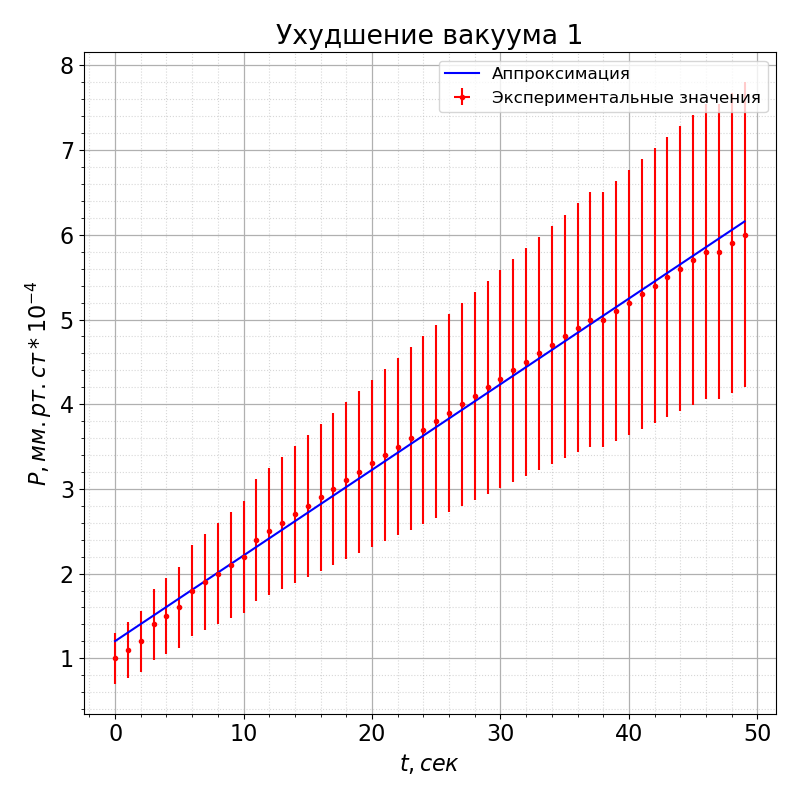
\includegraphics[width=1\linewidth]{graphs/rise1.png}
                    \captionof{figure}{Ухудшение вакуума 1}
                    \label{rise1}
                \end{minipage}
                \begin{minipage}{0.45\textwidth}
                    \centering
                    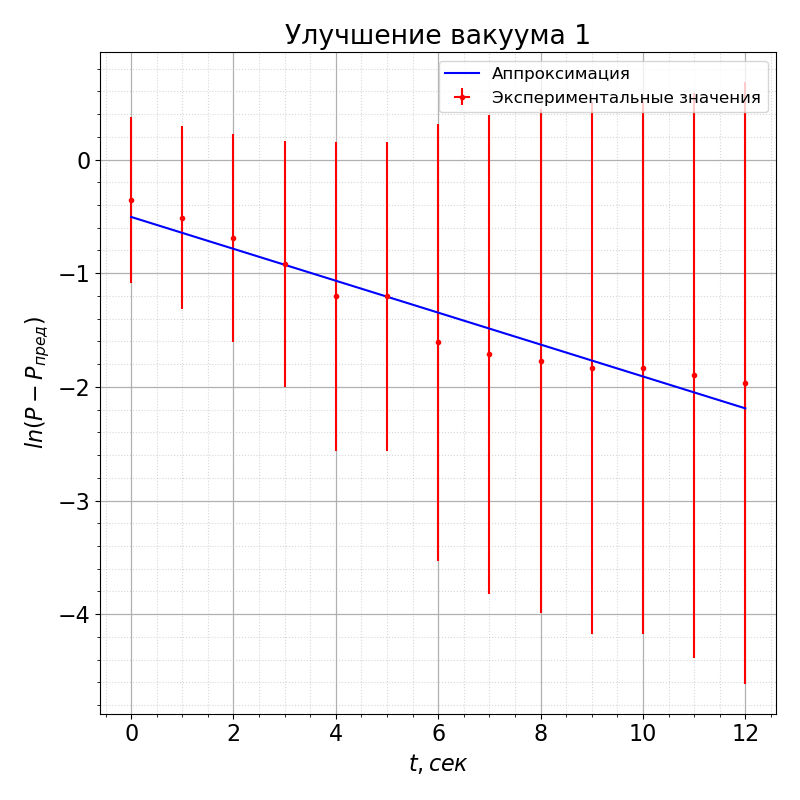
\includegraphics[width=1\linewidth]{graphs/fall1.png}
                    \captionof{figure}{Улучшение вакуума 1}
                    \label{fall1}
                \end{minipage}
            \end{figure}

            \begin{figure}[ht]
                \centering
                \begin{minipage}{0.45\textwidth}
                    \centering
                    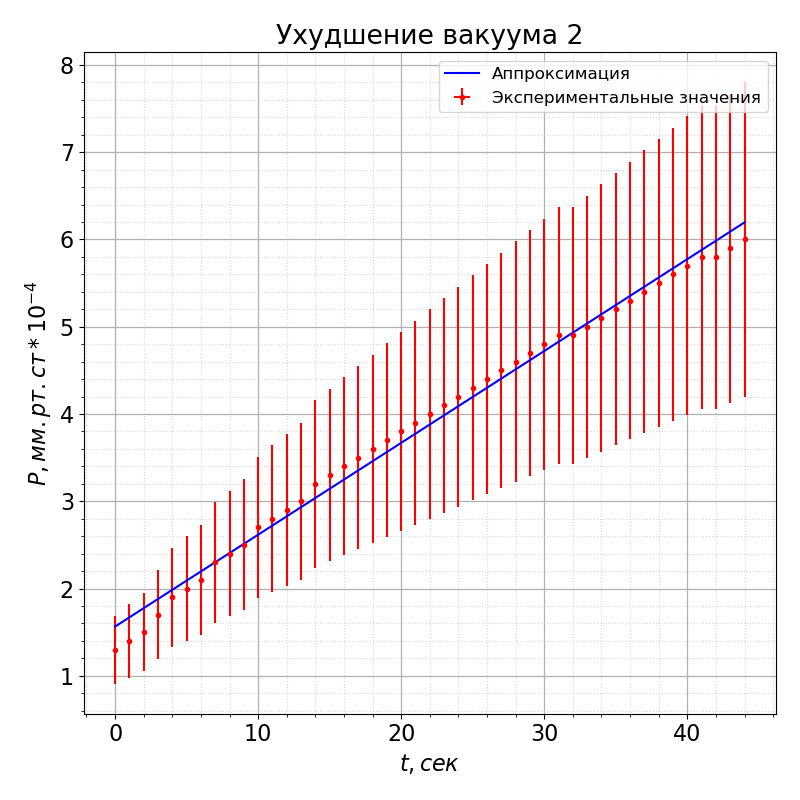
\includegraphics[width=1\linewidth]{graphs/rise2.png}
                    \captionof{figure}{Ухудшение вакуума 2}
                    \label{rise2}
                \end{minipage}
                \begin{minipage}{0.45\textwidth}
                    \centering
                    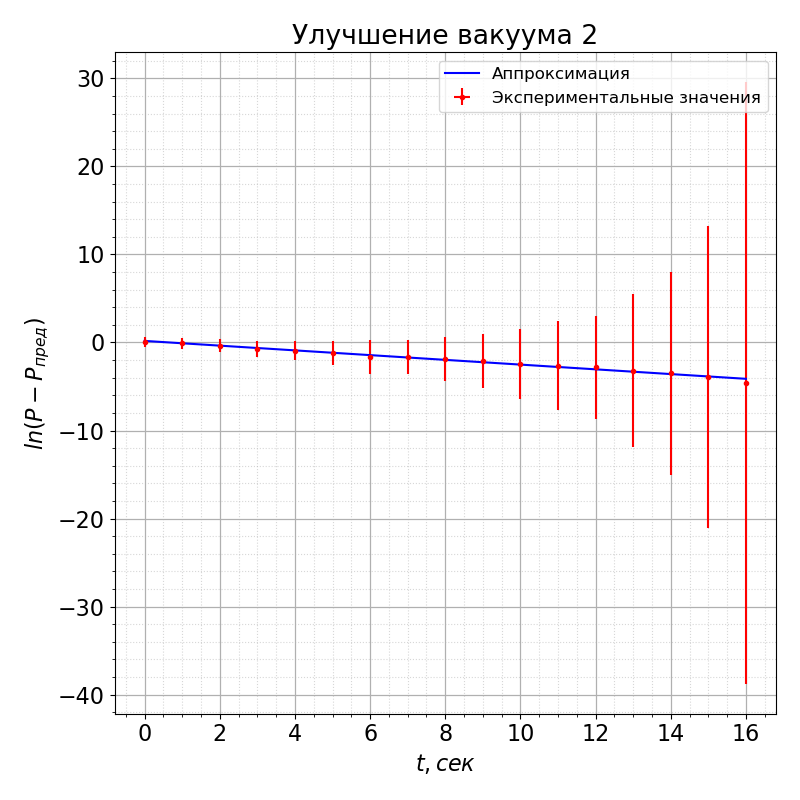
\includegraphics[width=1\linewidth]{graphs/fall2.png}
                    \captionof{figure}{Улучшение вакуума 2}
                    \label{fall2}
                \end{minipage}
            \end{figure}

            3. Из графиков \ref{fall1} и \ref{fall2} по МНК получаем коэффициенты прямых:

            \begin{align*}
                k_1 &= (-0.140 \pm 0.012)~с^{-1}\\
                k_2 &= (-0.269 \pm 0.008)~с^{-1}\\
                k_{ср} &= (-0.20 \pm 0.07)~с^{-1}
            \end{align*}

            4. Рассчитываем скорость откачки

            Из формулы (\ref{W}) приборная погрешность скорости откачки:

            \begin{align*}
                \sigma_W^{приб} &= W \sqrt{\left( \frac{\sigma_{V_{вв}}}{V_{вв}} \right)^2 + \left( \frac{\sigma_{t}}{t} \right)^2 + \left( \frac{\sigma_{P - P_{пред}}}{(P - P_{пред}) ln(P - P_{пред})} \right)^2}\\
                \sigma_W &= \sqrt{{\sigma_W^{случ}}^2 + {\sigma_W^{приб}}^2} = 50~см^3/с
            \end{align*}

            Итого:

            \begin{align*}
                W &= -k_{ср} * V_{вв} = (230 \pm 50)~см^3/с
            \end{align*}

        \subsubsection{Оцениваем величину потока газа, поступающего из насоса назад в откачиваемую систему}

            Воспользуемся уравнением

            \begin{align*}
                V_{вв} dP &= (Q_д + Q_и)dt
            \end{align*}

            Получаем зависимость (k - средний из двух коэффициентов наклона прямых графиков в координатах $P(t)$ при ухудшении вакуума)

            \begin{align*}
                Q_д + Q_и &= k V_{вв}
            \end{align*}

            \begin{align*}
                k_1 &= (1.011 \pm 0.009) * 10^{-5} мм.рт.ст/с\\
                k_2 &= (1.053 \pm 0.015) * 10^{-5} мм.рт.ст/с\\
                k &= (1.032 \pm 0.024) * 10^{-5} мм.рт.ст/с
            \end{align*}

            Зная также, что $P_{пред}W = Q_д + Q_и + Q_н$, получим

            \begin{align*}
                Q_н &= P_{пред} W - k V_{вв} = 7 * 10^{-3}~мм.рт.ст*см^3/с\\
                \sigma_{Q_н}^{приб} &= \sqrt{ \left( \frac{P V_{вв}}{t} \right)^2 \left( \left( \frac{\sigma_P}{P} \right)^2 + \left( \frac{\sigma_{V_{вв}}}{V_{вв}} \right)^2 + \left( \frac{\sigma_t}{t} \right)^2 \right) + \left( P_{пред} W \right)^2 \left( \left( \frac{\sigma_{P_{пред}}}{P_{пред}} \right)^2 + \left( \frac{\sigma_W}{W} \right)^2 \right)}\\
                \sigma_{Q_н} &= 7 * 10^{-3}~мм.рт.ст*см^3/с\\
            \end{align*}

        \subsubsection{Оцениваем пропускную способность трубки от высоковакуумного баллона до насоса}

            Параметры трубки: $L = (10 \pm 0.1)~см$, $d = (0.8 \pm 0.1)~см$

            $T = (295.2 \pm 0.1)~К$

            Вычислим по формуле (\ref{C_trubki}) и соответствующей формуле для приборной погрешности.

            $C_{тр} = (600 \pm 500)~см^3/с$

            Как видим, полученное значение вполне согласуется с рассчитанной ранее производительностью насоса.

        \subsubsection{Вводим искуственную течь в систему}

            То есть открываем кран между форвакуумной и высоковакуумными частями установки. В результате через 3-5 минут в обеих частях установились разные давления:

            \begin{align*}
                P_{уст} &= (2.0 \pm 0.6)*10^{-4}~мм.рт.ст\\
                P_{фв} &= (1.0 \pm 0.3)*10^{-3}~мм.рт.ст
            \end{align*}

        \subsubsection{Рассчитаем производительность диффузионного насоса через $P_{уст}$ и $P_{фв}$}

		    $$P_{пред}W = Q_1, \quad P_{уст}W = Q_1 + \frac{(PV)_{кап}}{dt}$$

            $$W = \frac{C_{тр} P_{фв}}{P_{уст} - P_{пред}}$$

            Аналогично предыдущим пунктам рассчитываем полную погрешность и само значение:

            $$W = (5 \pm 4)~л/c$$

            Напомним, что ранее мы получили производительность насоса $W = (0.23 \pm 0.05)~л/с$.

    \section{Вывод}

        Измерили объёмы форвакуумной и высоковакуумной частей установки. Определили скорость откачки системы в стационарном режиме, а также по ухудшению и по улучшению вакуума. Полученные результаты сравнимы в пределах погрешностей.

\end{document}
